%=======================================================================
% mmae450/tex/lectures/lecture_fvm_1D_intro.tex
% Standalone Beamer deck that inputs an existing Chapter 5 .tikz figure
% located in: mmae450/tex/figures/lectures/
%
% IMPORTANT:
% The .tikz file itself does: \input{tex/preamble/tikz_house_styles.tex}
% so we add the repo root to TeX's input search path using \input@path.
%=======================================================================


\documentclass[aspectratio=169]{beamer}

\makeatletter
\def\input@path{{../figures/lectures/}}
\makeatother

% --- Your beamer styling (adjust path/name if yours differs)
\input{../preamble/beamer_styles.tex}

% --- TikZ (beamer_styles.tex may already load it; harmless if duplicated)
\usepackage{tikz}
\usepackage{graphicx}
\usetikzlibrary{arrows.meta,calc,positioning,decorations.pathreplacing}

% --- Make sure TeX can resolve paths like tex/preamble/... used INSIDE the .tikz
% From mmae450/tex/lectures, the repo root is ../../


\title{Finite Element Method}
\subtitle{2D Elasticity Problems}
\author{MMAE 450}
\date{}

\begin{document}

\makeatletter
\def\input@path{{../../}{../}{./}}
\makeatother

% ----------------------------------------------------------------------
\begin{frame}
  \titlepage
\end{frame}
%=================================================

%==================== Slide 1 ====================
\begin{frame}{Finite Element Method for Solid Mechanics}

\begin{columns}

\column{0.5\textwidth}

\begin{itemize}
\item Plane stress / plane strain formulation
\item Weak form
\item Linear triangular elements
\item Assembly of the global stiffness matrix
\end{itemize}

\bigskip
Goal: derive the matrix system

\[
\mathbf{K}\mathbf{d}=\mathbf{F}
\]

\column{0.5\textwidth}

\centering

\includegraphics[width=\textwidth]{fe_contour.png}

\end{columns}

\end{frame}

%==================== Slide 2 ====================
\begin{frame}{Equilibrium Equations}

\begin{columns}[T,onlytextwidth]

\column{0.58\textwidth}

\textbf{Static equilibrium in a solid:}

\[
\boldsymbol{\nabla}\cdot\boldsymbol{\sigma}+\mathbf{b}=0
\qquad \text{in } \Omega
\]

\medskip
\textbf{Boundary conditions:}

\[
u_i = u_i^* \qquad \text{on } \Gamma_u
\]

\[
t_i = t_i^* \qquad \text{on } \Gamma_t
\]

where

\[
t_i = \sigma_{ij} n_j
\]

\medskip
\begin{itemize}
\item $\Gamma_u$: displacement boundary
\item $\Gamma_t$: traction boundary
\end{itemize}

\column{0.42\textwidth}

\centering

\includegraphics[width=0.95\textwidth]{chap05_fig03_potato_momentum.png}

\vspace{1mm}
{\footnotesize Momentum balance over an arbitrary region}

\end{columns}

\end{frame}


%==================== Slide 3 ====================

%==================== Slide 2 ====================
\begin{frame}{Weak Form}

Multiply the equilibrium equation by a test function $w_i$:

\[
\int_\Omega
w_i(\sigma_{ij,j}+b_i)\,d\Omega = 0
\]

\textbf{Test function requirements:}

\begin{itemize}
\item $w_i = 0$ on $\Gamma_u$
\item otherwise $w_i$ has the same continuity as the displacement field
\end{itemize}

Such test functions are called \textbf{kinematically admissible}.

\end{frame}

%==================== Slide 4 ====================
\begin{frame}{Weak Form}

Applying the divergence theorem gives

\[
\int_\Omega \sigma_{ij} w_{i,j}\,d\Omega
=
\int_{\Gamma} t_i w_i\,d\Gamma
+
\int_\Omega b_i w_i\,d\Omega
\]

Using the boundary conditions:

\[
\int_\Omega \sigma_{ij} w_{i,j}\,d\Omega
=
\int_{\Gamma_t} t_i^* w_i\,d\Gamma
+
\int_\Omega b_i w_i\,d\Omega
\]

because $w_i=0$ on $\Gamma_u$.

\end{frame}

%==================== Slide 5 ====================
\begin{frame}{Product Rule Identity}

To transform the integral statement we use the identity

\[
(\sigma_{ij} w_i)_{,j}
=
\sigma_{ij,j} w_i
+
\sigma_{ij} w_{i,j}.
\]

Rearranging,

\[
\sigma_{ij,j} w_i
=
(\sigma_{ij} w_i)_{,j}
-
\sigma_{ij} w_{i,j}.
\]

This identity shifts the derivative from the stress field
to the test function.

\bigskip

This step reduces the continuity requirement on $\sigma_{ij}$.

\end{frame}

%==================== Slide 6 ====================
\begin{frame}{Applying the Identity}

Start with the statement

\[
\int_\Omega w_i (\sigma_{ij,j}+b_i) \, d\Omega = 0.
\]

Substitute

\[
\sigma_{ij,j} w_i
=
(\sigma_{ij} w_i)_{,j}
-
\sigma_{ij} w_{i,j}
\]

to obtain

\[
\int_\Omega
(\sigma_{ij} w_i)_{,j} d\Omega
-
\int_\Omega
\sigma_{ij} w_{i,j} d\Omega
+
\int_\Omega
b_i w_i d\Omega
=0.
\]

\end{frame}







%==================== Slide 8 ====================
\begin{frame}{Weak Form of the Equilibrium Equations}

Applying the divergence theorem gives

\[
\int_\Omega
\sigma_{ij} w_{i,j}\, d\Omega
=
\int_{\Gamma}
t_i w_i\, d\Gamma
+
\int_\Omega
b_i w_i\, d\Omega
\]

Applying the boundary conditions on $\Gamma = \Gamma_u + \Gamma_t$:

\[
w_i = 0 \quad \text{on } \Gamma_u
\]

gives

\[
\boxed{
\int_\Omega
\sigma_{ij} w_{i,j}\, d\Omega
=
\int_{\Gamma_t}
t_i^* w_i\, d\Gamma
+
\int_\Omega
b_i w_i\, d\Omega
}
\]

\end{frame}
%==================== Slide 9 ====================
\begin{frame}{Finite Element Approximation}

The weak form involves two unknown fields:

\[
u_i(x,y) \qquad \text{and} \qquad w_i(x,y)
\]

In the finite element method we approximate these fields
using shape functions.

\bigskip

\textbf{Displacement approximation}

\[
u_i^e(x,y) = N_a(x,y)\, u_i^a
\]

\textbf{Test function approximation}

\[
w_i^e(x,y) = N_a(x,y)\, w_i^a
\]

\bigskip

\begin{itemize}
\item $N_a(x,y)$ : element shape functions
\item $u_i^a$ : nodal displacement components
\item $w_i^a$ : nodal values of the test function
\end{itemize}

Using the same shape functions for both fields is called
the \textbf{Galerkin method}.

\end{frame}

%==================== Slide 10 ====================
\begin{frame}{Three-Node Triangular Element}

\centering

\begin{tikzpicture}[scale=1.35]

% Nodes
\coordinate (n1) at (0,0);
\coordinate (n2) at (4.2,0);
\coordinate (n3) at (1.5,2.8);

% Triangle
\draw[thick] (n1) -- (n2) -- (n3) -- cycle;

% Node markers
\fill (n1) circle (2pt);
\fill (n2) circle (2pt);
\fill (n3) circle (2pt);

% Node labels
\node[below left]  at (n1) {1};
\node[below right] at (n2) {2};
\node[above]       at (n3) {3};

% Nodal displacement labels
\node[left,  xshift=-4mm] at (n1) {$\mathbf{u}^1$};
\node[right, xshift= 4mm] at (n2) {$\mathbf{u}^2$};
\node[above, yshift= 4mm] at (n3) {$\mathbf{u}^3$};

% Interior label
\node at (1.95,1.0) {$\mathbf{u}_e(x,y)$};

\end{tikzpicture}

\bigskip

For a linear triangular element, the displacement field inside the element
is interpolated from the nodal displacement vectors
\[
\mathbf{u}^1,\qquad \mathbf{u}^2,\qquad \mathbf{u}^3.
\]

\end{frame}
%==================== Slide 11 ====================
%==================== Slide 12 ====================
\begin{frame}{Matrix Form of the Displacement Field}

The nodal displacement vectors are stored in the element displacement vector

\[
\underset{6\times 1}{\mathbf{d}_e} =
\begin{bmatrix}
u_x^1 \\
u_y^1 \\
u_x^2 \\
u_y^2 \\
u_x^3 \\
u_y^3
\end{bmatrix}
\]

The displacement field inside the element is then written as

\[
\mathbf{u}_e(x,y)=\mathbf{N}_e(x,y)\mathbf{d}_e
\]

where

\[
\mathbf{N}_e =
\begin{bmatrix}
N_1 & 0 & N_2 & 0 & N_3 & 0 \\
0 & N_1 & 0 & N_2 & 0 & N_3
\end{bmatrix}.
\]

\end{frame}


%==================== Slide 13 ====================
%==================== Slide ====================
\begin{frame}{Internal Work Term for Plane Stress}

For plane stress, the only nonzero stress components are

\[
\sigma_{11},\qquad \sigma_{22},\qquad \sigma_{12}=\sigma_{21}.
\]

Thus

\[
\sigma_{ij} w_{i,j}
=
\sigma_{11} w_{1,1}
+\sigma_{22} w_{2,2}
+\sigma_{12}(w_{1,2}+w_{2,1}).
\]

Define the virtual strain vector

\[
\delta\boldsymbol{\varepsilon}_e=
\begin{bmatrix}
w_{1,1}\\[4pt]
w_{2,2}\\[4pt]
w_{1,2}+w_{2,1}
\end{bmatrix},
\qquad
\boldsymbol{\sigma}_e=
\begin{bmatrix}
\sigma_{11}\\[4pt]
\sigma_{22}\\[4pt]
\sigma_{12}
\end{bmatrix}.
\]

Then

\[
\sigma_{ij} w_{i,j}
=
\delta\boldsymbol{\varepsilon}_e^{\,T}\boldsymbol{\sigma}_e.
\]

\end{frame}
%==================== Slide 14 ====================

%==================== Slide ====================
\begin{frame}{Hooke's Law for Plane Stress}

Hooke's law for plane stress may be written as

\[
\begin{bmatrix}
\sigma_{11}\\
\sigma_{22}\\
\sigma_{12}
\end{bmatrix}
=
\frac{E}{1-\nu^2}
\begin{bmatrix}
1 & \nu & 0\\
\nu & 1 & 0\\
0 & 0 & \dfrac{1-\nu}{2}
\end{bmatrix}
\begin{bmatrix}
\epsilon_{11}\\
\epsilon_{22}\\
\gamma_{12}
\end{bmatrix}
\]

or


\[
\boldsymbol{\sigma}_e=\mathbf{C}_e\boldsymbol{\varepsilon}_e
\]

where

\[
\boldsymbol{\sigma}_e=
\begin{bmatrix}
\sigma_{11}\\
\sigma_{22}\\
\sigma_{12}
\end{bmatrix},
\qquad
\boldsymbol{\varepsilon}_e=
\begin{bmatrix}
\epsilon_{11}\\
\epsilon_{22}\\
\gamma_{12}
\end{bmatrix},
\qquad
\mathbf{C}_e=
\frac{E}{1-\nu^2}
\begin{bmatrix}
1 & \nu & 0\\
\nu & 1 & 0\\
0 & 0 & \dfrac{1-\nu}{2}
\end{bmatrix}
\]



\end{frame}
%==================== Slide ====================
\begin{frame}{Strain–Displacement Relations}

The strain components are related to the displacement field
\[
\mathbf{u}(x,y) =
\begin{bmatrix}
u_1(x,y)\\
u_2(x,y)
\end{bmatrix}.
\]

For small deformations,

\[
\epsilon_{11} = \frac{\partial u_1}{\partial x_1},
\qquad
\epsilon_{22} = \frac{\partial u_2}{\partial x_2},
\qquad
\gamma_{12} =
\frac{\partial u_1}{\partial x_2}
+
\frac{\partial u_2}{\partial x_1}.
\]

Collecting these into vector form gives

\[
\boldsymbol{\varepsilon}=
\begin{bmatrix}
\epsilon_{11}\\
\epsilon_{22}\\
\gamma_{12}
\end{bmatrix}
=
\begin{bmatrix}
u_{1,1}\\
u_{2,2}\\
u_{1,2}+u_{2,1}
\end{bmatrix}.
\]

\end{frame}
%==============================================

%==================== Slide ====================
\begin{frame}{Strain and Virtual Strain}

Recall the strain vector

\[
\boldsymbol{\varepsilon}=
\begin{bmatrix}
\epsilon_{11}\\
\epsilon_{22}\\
\gamma_{12}
\end{bmatrix}
=
\begin{bmatrix}
u_{1,1}\\
u_{2,2}\\
u_{1,2}+u_{2,1}
\end{bmatrix}.
\]

Similarly, the virtual strain associated with the test function is

\[
\delta\boldsymbol{\varepsilon}=
\begin{bmatrix}
w_{1,1}\\
w_{2,2}\\
w_{1,2}+w_{2,1}
\end{bmatrix}.
\]

Notice the identical structure of these two expressions.

\bigskip

Using the finite element approximations,

\[
\boxed{\boldsymbol{\varepsilon}_e = \mathbf{B}_e \mathbf{d}_e},
\qquad
\boxed{\delta\boldsymbol{\varepsilon}_e = \mathbf{B}_e \mathbf{w}_e}.
\]

\end{frame}


%==================== Slide ====================
\begin{frame}{Internal Virtual Work for a Single Element}

For a single element \( \Omega_e \), the internal virtual work term is

\[
\int_{\Omega_e} \sigma_{ij}\, w_{i,j}\, d\Omega
=
\int_{\Omega_e}
\delta\boldsymbol{\varepsilon}_e^{\,T}\boldsymbol{\sigma}_e
\, d\Omega
\]

Using

\[
\boldsymbol{\sigma}_e=\mathbf{C}_e\boldsymbol{\varepsilon}_e,
\qquad
\boldsymbol{\varepsilon}_e=\mathbf{B}_e\mathbf{d}_e,
\qquad
\delta\boldsymbol{\varepsilon}_e=\mathbf{B}_e\mathbf{w}_e,
\]

we obtain



\[
=
\int_{\Omega_e}
(\mathbf{B}_e\mathbf{w}_e)^T
\mathbf{C}_e
(\mathbf{B}_e\mathbf{d}_e)
\, d\Omega
\]

\[
=
\mathbf{w}_e^T
\left(
\int_{\Omega_e}
\mathbf{B}_e^T \mathbf{C}_e \mathbf{B}_e
\, d\Omega
\right)
\mathbf{d}_e.
\]

\end{frame}



%==================== Slide 15 ====================
\begin{frame}{Strain--Displacement Matrix for a Linear Triangle}

The strain vector is

\[
\boldsymbol{\varepsilon}_e=
\begin{bmatrix}
\epsilon_{11}\\
\epsilon_{22}\\
\gamma_{12}
\end{bmatrix}
=
\begin{bmatrix}
u_{1,1}\\
u_{2,2}\\
u_{1,2}+u_{2,1}
\end{bmatrix}
=
\mathbf{B}_e\mathbf{d}_e,
\]

where

\[
\mathbf{B}_e=
\begin{bmatrix}
N_{1,1} & 0       & N_{2,1} & 0       & N_{3,1} & 0\\
0       & N_{1,2} & 0       & N_{2,2} & 0       & N_{3,2}\\
N_{1,2} & N_{1,1} & N_{2,2} & N_{2,1} & N_{3,2} & N_{3,1}
\end{bmatrix}.
\]

For the linear triangle, the derivatives of the shape functions are constant,
so \(\mathbf{B}_e\) is constant within the element.

\end{frame}

%=================================================
%==================== Slide ====================
\begin{frame}{Body Force Contribution}

The body force term in the weak form is

\[
\int_{\Omega_e} w_i b_i \, d\Omega.
\]

Using the finite element approximation for the test function

\[
\mathbf{w}(x,y)=\mathbf{N}_e(x,y)\mathbf{w}_e,
\]

we obtain

\[
\int_{\Omega_e} w_i b_i \, d\Omega
=
\int_{\Omega_e}
(\mathbf{N}_e \mathbf{w}_e)^T \mathbf{b}
\, d\Omega.
\]

Rearranging gives

\[
=
\mathbf{w}_e^T
\left(
\int_{\Omega_e}
\mathbf{N}_e^T \mathbf{b}
\, d\Omega
\right).
\]

\end{frame}

%=====================================
%==================== Slide ====================
\begin{frame}{Traction Boundary Contribution}

The traction term in the weak form is

\[
\int_{\Gamma_t^e} w_i t_i^* \, d\Gamma.
\]

Using the finite element approximation

\[
\mathbf{w}(x,y)=\mathbf{N}_e(x,y)\mathbf{w}_e,
\]

we obtain

\[
\int_{\Gamma_t^e} w_i t_i^* \, d\Gamma
=
\int_{\Gamma_t^e}
(\mathbf{N}_e \mathbf{w}_e)^T \mathbf{t}^*
\, d\Gamma.
\]

Rearranging gives

\[
=
\mathbf{w}_e^T
\left(
\int_{\Gamma_t^e}
\mathbf{N}_e^T \mathbf{t}^*
\, d\Gamma
\right).
\]

\end{frame}
%==================== Slide 15 ====================

\begin{frame}{Total Element Contribution to the Weak Form}

Substituting all of the finite element approximations into the weak form gives

\[
\mathbf{w}_e^T
\left(
\int_{\Omega_e}
\mathbf{B}_e^T
\mathbf{C}_e
\mathbf{B}_e
\, d\Omega
\right)
\mathbf{d}_e
=
\mathbf{w}_e^T
\left(
\int_{\Omega_e}
\mathbf{N}_e^T \mathbf{b}
\, d\Omega
+
\int_{\Gamma_t^e}
\mathbf{N}_e^T \mathbf{t}^*
\, d\Gamma
\right).
\]

This equation represents the contribution of a single element
to the global weak form.

\end{frame}


%==================== Slide 15 ====================

\begin{frame}{Element Stiffness Matrix and Load Vector}

Define the element stiffness matrix

\[
\boxed{
\mathbf{K}_e
=
\int_{\Omega_e}
\mathbf{B}_e^T
\mathbf{C}_e
\mathbf{B}_e
\, d\Omega
}
\]

and the element load vector

\[
\boxed{
\mathbf{f}_e
=
\int_{\Omega_e}
\mathbf{N}_e^T \mathbf{b}
\, d\Omega
+
\int_{\Gamma_t^e}
\mathbf{N}_e^T \mathbf{t}^*
\, d\Gamma
}.
\]

The element equation becomes

\[
\mathbf{w}_e^T \mathbf{K}_e \mathbf{d}_e
=
\mathbf{w}_e^T \mathbf{f}_e.
\]

\end{frame}

%=============================================
\begin{frame}{Assembly of the Global System}

The weak form must hold for all elements in the mesh.

Summing the element contributions gives

\[
\sum_e
\mathbf{w}_e^T
\mathbf{K}_e
\mathbf{d}_e
=
\sum_e
\mathbf{w}_e^T
\mathbf{f}_e.
\]

Using Boolean assembly matrices

\[
\mathbf{d}_e=\mathbf{L}_e\mathbf{d},
\qquad
\mathbf{w}_e=\mathbf{L}_e\mathbf{w},
\]

we obtain

\[
\mathbf{w}^T
\left(
\sum_e
\mathbf{L}_e^T
\mathbf{K}_e
\mathbf{L}_e
\right)
\mathbf{d}
=
\mathbf{w}^T
\left(
\sum_e
\mathbf{L}_e^T
\mathbf{f}_e
\right).
\]

\end{frame}

%==============================
\begin{frame}{Global Finite Element Equations}

Since the equation must hold for all admissible $\mathbf{w}$,

\[
\boxed{
\mathbf{K}\mathbf{d}=\mathbf{F}
}
\]

where

\[
\mathbf{K}
=
\sum_e
\mathbf{L}_e^T
\mathbf{K}_e
\mathbf{L}_e,
\qquad
\mathbf{F}
=
\sum_e
\mathbf{L}_e^T
\mathbf{f}_e.
\]

\end{frame}
%=============================================
\begin{frame}{Boolean Matrix and Element Assembly}

\begin{columns}[T,onlytextwidth]

%---------------------------------
% Left column: mesh
%---------------------------------
\column{0.36\textwidth}

\centering
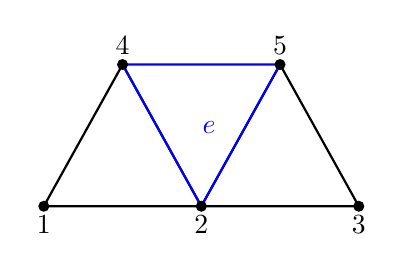
\begin{tikzpicture}[scale=1.0]

\coordinate (n1) at (0,0);
\coordinate (n2) at (2,0);
\coordinate (n3) at (4,0);
\coordinate (n4) at (1,1.8);
\coordinate (n5) at (3,1.8);

\draw[thick] (n1)--(n2)--(n4)--cycle;
\draw[thick] (n2)--(n3)--(n5)--cycle;
\draw[thick,blue] (n2)--(n5)--(n4)--cycle;

\fill (n1) circle (2pt);
\fill (n2) circle (2pt);
\fill (n3) circle (2pt);
\fill (n4) circle (2pt);
\fill (n5) circle (2pt);

\node[below] at (n1) {1};
\node[below] at (n2) {2};
\node[below] at (n3) {3};
\node[above] at (n4) {4};
\node[above] at (n5) {5};

\node[blue] at (2.1,1.0) {$e$};

\end{tikzpicture}

\medskip
Element \(e\) connects nodes \((2,4,5)\).

%---------------------------------
% Right column: algebra
%---------------------------------
\column{0.64\textwidth}

\scriptsize

The global displacement vector is

\[
\mathbf{d}
=
\begin{bmatrix}
u_1^1 & u_2^1 & u_1^2 & u_2^2 & u_1^3 &
u_2^3 & u_1^4 & u_2^4 & u_1^5 & u_2^5
\end{bmatrix}^{T}.
\]

For element \(e=(2,4,5)\), the element displacement vector is

\[
\mathbf{d}_e
=
\begin{bmatrix}
u_1^2 & u_2^2 & u_1^4 & u_2^4 & u_1^5 & u_2^5
\end{bmatrix}^{T}.
\]

Thus,

\[
\boxed{
\mathbf{d}_e=\mathbf{L}_e\,\mathbf{d}
}
\]

where \(\mathbf{L}_e\) is the Boolean matrix that selects the
degrees of freedom associated with element \(e\).

\end{columns}

\end{frame}
%===============================================
%==================== Slide ====================

%==================== Slide ====================
\begin{frame}{Boolean Matrix Mapping}

The element displacement vector is obtained from the global vector by

\[
\mathbf{d}_e = \mathbf{L}_e \mathbf{d}.
\]

For element \(e=(2,4,5)\),

\[
\begin{bmatrix}
u_1^2 \\
u_2^2 \\
u_1^4 \\
u_2^4 \\
u_1^5 \\
u_2^5
\end{bmatrix}
=
\begin{bmatrix}
0&0&1&0&0&0&0&0&0&0\\
0&0&0&1&0&0&0&0&0&0\\
0&0&0&0&0&0&1&0&0&0\\
0&0&0&0&0&0&0&1&0&0\\
0&0&0&0&0&0&0&0&1&0\\
0&0&0&0&0&0&0&0&0&1
\end{bmatrix}
\begin{bmatrix}
u_1^1\\
u_2^1\\
u_1^2\\
u_2^2\\
u_1^3\\
u_2^3\\
u_1^4\\
u_2^4\\
u_1^5\\
u_2^5
\end{bmatrix}.
\]

\end{frame}
%==================== Slide ====================








%=============================================













































%=========================================
\begin{frame}{Shape Functions for the Triangle (CST Element)}

For a three-node linear triangular element, the displacement field is

\[
\mathbf{u}_e(x,y)=\mathbf{N}_e(x,y)\mathbf{d}_e
\]

where the shape-function matrix is

\[
\mathbf{N}_e=
\begin{bmatrix}
N_1 & 0 & N_2 & 0 & N_3 & 0\\
0 & N_1 & 0 & N_2 & 0 & N_3
\end{bmatrix}.
\]

The functions \(N_1(x,y), N_2(x,y), N_3(x,y)\) are the
\textbf{linear shape functions} associated with the three nodes.

\end{frame}
%=============================================
%==================== Slide ====================
\begin{frame}{Linear Shape Functions for a Triangle}

For a three-node triangular element, each shape function is a
linear polynomial in \(x\) and \(y\):

\[
N_a(x,y)=\frac{1}{2A_e}\left(\alpha_a+b_a x+c_a y\right),
\qquad a=1,2,3.
\]

The coefficients depend only on the nodal coordinates

\[
(x_1,y_1),\qquad (x_2,y_2),\qquad (x_3,y_3).
\]

The element area is

\[
A_e=
\frac12
\begin{vmatrix}
1 & x_1 & y_1\\
1 & x_2 & y_2\\
1 & x_3 & y_3
\end{vmatrix}.
\]

\end{frame}
%=============================================
%==================== Slide ====================
\begin{frame}{Coefficients \(\alpha_a\)}

The constants \( \alpha_a \) are

\[
\alpha_1 = x_2y_3 - x_3y_2
\]

\[
\alpha_2 = x_3y_1 - x_1y_3
\]

\[
\alpha_3 = x_1y_2 - x_2y_1
\]

These depend only on the element nodal coordinates.

\end{frame}

%=============================================
%==================== Slide ====================
\begin{frame}{Coefficients \(b_a\) and \(c_a\)}

The remaining coefficients are

\[
b_1=y_2-y_3,\qquad b_2=y_3-y_1,\qquad b_3=y_1-y_2
\]

\[
c_1=x_3-x_2,\qquad c_2=x_1-x_3,\qquad c_3=x_2-x_1
\]

For a linear triangular element the derivatives of the shape functions
are constant within the element.

\end{frame}

%=============================================
\begin{frame}{Area Coordinate Interpretation}

\begin{columns}[T,onlytextwidth]

%---------------------------------
% Left: triangle
%---------------------------------
\column{0.55\textwidth}

\centering
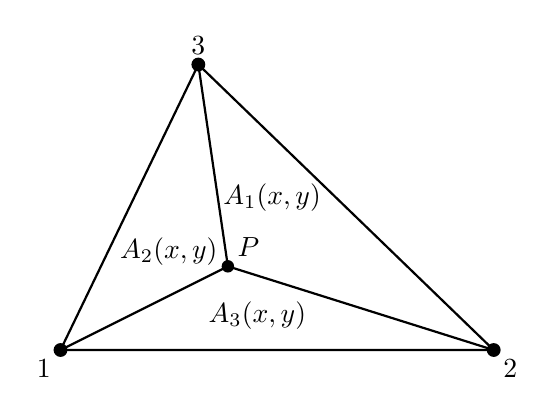
\begin{tikzpicture}[scale=1.25]

% Triangle nodes
\coordinate (n1) at (0,0);
\coordinate (n2) at (4.4,0);
\coordinate (n3) at (1.4,2.9);

% Interior point
\coordinate (P) at (1.7,0.85);

% Outer triangle
\draw[thick] (n1) -- (n2) -- (n3) -- cycle;

% Subtriangle lines
\draw[thick] (P) -- (n1);
\draw[thick] (P) -- (n2);
\draw[thick] (P) -- (n3);

% Nodes
\fill (n1) circle (2pt);
\fill (n2) circle (2pt);
\fill (n3) circle (2pt);
\fill (P)  circle (1.8pt);

% Node labels
\node[below left]  at (n1) {1};
\node[below right] at (n2) {2};
\node[above]       at (n3) {3};

% Point label
\node[above right] at (P) {$P$};

% Area labels
\node at (2.15,1.55) {$A_1(x,y)$};
\node at (1.1,1.00) {$A_2(x,y)$};
\node at (2.0,0.35) {$A_3(x,y)$};

\end{tikzpicture}

%---------------------------------
% Right: identities
%---------------------------------
\column{0.45\textwidth}

\[
\boxed{N_1+N_2+N_3=1}
\]

\[
N_a(x_b,y_b)=\delta_{ab}
\]

\medskip

\begin{itemize}
\item Partition of unity
\item Interpolation property
\end{itemize}

\end{columns}

\vspace{4mm}

Let \(A_e\) be the total area of the element.  
The shape functions may be written as

\[
N_1(x,y)=\frac{A_1(x,y)}{A_e},
\qquad
N_2(x,y)=\frac{A_2(x,y)}{A_e},
\qquad
N_3(x,y)=\frac{A_3(x,y)}{A_e}.
\]

\end{frame}

%=============================================
%==================== Slide ====================
\begin{frame}{Derivatives of the Shape Functions}

For a linear triangular element,

\[
N_a(x,y)=\frac{1}{2A_e}\left(\alpha_a+b_a x+c_a y\right).
\]

Taking derivatives gives

\[
\frac{\partial N_a}{\partial x}=\frac{b_a}{2A_e},
\qquad
\frac{\partial N_a}{\partial y}=\frac{c_a}{2A_e}.
\]

Thus the derivatives of the shape functions are constant
throughout the element.

\bigskip

This is why the element is called the

\[
\boxed{\text{Constant Strain Triangle (CST)}}
\]

\end{frame}
%=============================================
%==================== Slide ====================
%==================== Slide ====================
\begin{frame}{Strain--Displacement Matrix \( \mathbf{B}_e \)}

Recall that

\[
\boldsymbol{\varepsilon}_e=
\begin{bmatrix}
\epsilon_{11}\\
\epsilon_{22}\\
\gamma_{12}
\end{bmatrix}
=
\begin{bmatrix}
u_{1,1}\\
u_{2,2}\\
u_{1,2}+u_{2,1}
\end{bmatrix}.
\]

Using the finite element displacement approximation, we obtain

\[
\boldsymbol{\varepsilon}_e=\mathbf{B}_e \mathbf{d}_e
\]

with

\[
\mathbf{B}_e=
\begin{bmatrix}
N_{1,1} & 0       & N_{2,1} & 0       & N_{3,1} & 0\\
0       & N_{1,2} & 0       & N_{2,2} & 0       & N_{3,2}\\
N_{1,2} & N_{1,1} & N_{2,2} & N_{2,1} & N_{3,2} & N_{3,1}
\end{bmatrix}.
\]

\end{frame}
%=============================================

%==================== Slide ====================
\begin{frame}{\( \mathbf{B}_e \) in Terms of Area and Nodal Coordinates}

Since

\[
N_{a,1}=\frac{b_a}{2A_e},
\qquad
N_{a,2}=\frac{c_a}{2A_e},
\]

we may write

\[
\mathbf{B}_e=
\frac{1}{2A_e}
\begin{bmatrix}
b_1 & 0   & b_2 & 0   & b_3 & 0\\
0   & c_1 & 0   & c_2 & 0   & c_3\\
c_1 & b_1 & c_2 & b_2 & c_3 & b_3
\end{bmatrix},
\]


Thus,

\[
\mathbf{B}_e=
\frac{1}{2A_e}
\begin{bmatrix}
y_2-y_3 & 0 & y_3-y_1 & 0 & y_1-y_2 & 0\\
0 & x_3-x_2 & 0 & x_1-x_3 & 0 & x_2-x_1\\
x_3-x_2 & y_2-y_3 & x_1-x_3 & y_3-y_1 & x_2-x_1 & y_1-y_2
\end{bmatrix}.
\]

\end{frame}
%======================================================
\begin{frame}{Computing the CST Element Matrices}

In the companion notebook we derive

\[
N_a(x,y)
\quad \rightarrow \quad
\mathbf{B}_e
\quad \rightarrow \quad
\mathbf{K}_e
\]

for the three-node triangular element.

\bigskip

The notebook symbolically computes

\[
\mathbf{B}_e =
\frac{1}{2A_e}
\begin{bmatrix}
y_2-y_3 & 0 & y_3-y_1 & 0 & y_1-y_2 & 0\\
0 & x_3-x_2 & 0 & x_1-x_3 & 0 & x_2-x_1\\
x_3-x_2 & y_2-y_3 & x_1-x_3 & y_3-y_1 & x_2-x_1 & y_1-y_2
\end{bmatrix}.
\]


\end{frame}
%===========================================
%==================== Slide ====================
\begin{frame}{Example Problem Used in the Notebook}

\begin{columns}[T,onlytextwidth]

%---------------------------------
% Left: mesh
%---------------------------------
\column{0.48\textwidth}

\centering

\includegraphics[width=0.95\textwidth]{fe_mesh.png}

%---------------------------------
% Right: description
%---------------------------------
\column{0.42\textwidth}

\footnotesize

\textbf{Geometry}
\begin{itemize}\itemsep2pt
\item Plate with a circular hole
\item Plane stress model
\end{itemize}

\textbf{Boundary Conditions}
\begin{itemize}\itemsep2pt
\item Left edge: \(u_x = 0\)
\item Bottom edge: \(u_y = 0\)
\item Right edge: traction free
\item Top edge: \(t_y = t_y^*, t_x=0\)
\end{itemize}

\textbf{Material}
\begin{itemize}\itemsep2pt
\item Young's modulus \(E\)
\item Poisson ratio \(\nu\)
\end{itemize}

\end{columns}

\end{frame}

%==================== Slide ====================
%==================== Slide ====================
%==================== Slide ====================
%==================== Slide ====================
%==================== Slide ====================
%==================== Slide ====================
\begin{frame}{Finite Element Method for Solids: Algorithm Summary}

\small Assumptions: small strains, linear elastic material, static equilibrium

\small

\begin{center}
\fbox{
\begin{minipage}{0.9\textwidth}

\small

\begin{enumerate}

\item Interpolate displacement:
$\mathbf{u}_e=\mathbf{N}_e\mathbf{d}_e$

\item Strain--displacement relation:
$\boldsymbol{\varepsilon}_e=\mathbf{B}_e\mathbf{d}_e$

\item Constitutive law:
$\boldsymbol{\sigma}_e=\mathbf{C}_e\boldsymbol{\varepsilon}_e$

\item Element matrices:
$\mathbf{K}_e=\int_{\Omega_e}\mathbf{B}_e^T\mathbf{C}_e\mathbf{B}_e\,d\Omega,\;
\mathbf{f}_e=\int_{\Omega_e}\mathbf{N}_e^T\mathbf{b}\,d\Omega+\int_{\Gamma_t^e}\mathbf{N}_e^T\mathbf{t}^*\,d\Gamma$

\item Assemble:
$\mathbf{K}\mathbf{d}=\mathbf{F}$

\item Solve for nodal displacements:
$\mathbf{d}$

\item Post-process:
$\boldsymbol{\varepsilon}_e=\mathbf{B}_e\mathbf{d}_e$, 
$\boldsymbol{\sigma}_e=\mathbf{C}_e\boldsymbol{\varepsilon}_e$

\end{enumerate}

\end{minipage}
}
\end{center}

\end{frame}



%==================== Slide ====================
\begin{frame}{Assembly of the Global System}

\begin{columns}[T,onlytextwidth]

%---------------------------------
% Left: assembly figure
%---------------------------------
\column{0.58\textwidth}

\centering
\resizebox{\textwidth}{!}{%
%===========================================================
% chap06_fig03_FE_assembly_colored.tikz  (HOUSE STYLE)
% Assembly of two element matrices into a global matrix
%===========================================================

\providecommand{\FigWidth}{11.0cm} % fallback only
\def\FigDesignWidth{12.0}          % design units across (gives comfortable margins)

\input{tex/preamble/tikz_house_styles.tex}

\begin{tikzpicture}[house]

  % Keep this figure from inheriting any huge wrapper fonts
  \tikzset{
    every node/.style={font=\normalsize, align=center},
    main/.style={font=\figMainFont, align=center},
    axis/.style={font=\figAxisFont, align=center},
    meshLine/.style={line width=0.9pt},
    highlight1/.style={blue, line width=1.4pt},
    highlight2/.style={red,  line width=1.4pt},
  }

  % --------------------------------------------------------
  % 1D mesh (top), centered
  % --------------------------------------------------------
  \coordinate (x1) at (-2.3,0);
  \coordinate (x2) at (0,0);
  \coordinate (x3) at (2.3,0);

  \draw[meshLine] (x1) -- (x2) -- (x3);
  \fill (x1) circle (2.0pt);
  \fill (x2) circle (2.0pt);
  \fill (x3) circle (2.0pt);

  \node[axis, below=3pt] at (x1) {$1$};
  \node[axis, below=3pt] at (x2) {$2$};
  \node[axis, below=3pt] at (x3) {$3$};

  \node[axis, above=3pt] at ($(x1)!0.5!(x2)$) {$e=1$};
  \node[axis, above=3pt] at ($(x2)!0.5!(x3)$) {$e=2$};

  \coordinate (meshcenter) at ($(x1)!0.5!(x3)$); % (0,0)

  % --------------------------------------------------------
  % Element matrices K1 and K2, under the mesh
  % --------------------------------------------------------
  \coordinate (Kpaircenter) at ($(meshcenter)+(0,-2.0)$);

  \node[main] (K1) at ($(Kpaircenter)+(-2.7,0)$)
  {$\displaystyle
    \mathbf{K}_1 =
    \begin{bmatrix}
      k_{11}^{(1)} & k_{12}^{(1)} \\
      k_{21}^{(1)} & k_{22}^{(1)}
    \end{bmatrix}$};

 % --- K1 row labels (moved up more)
\node[axis] at ($(K1.east)+(0.20,0.42)$) {$1$};
\node[axis] at ($(K1.east)+(0.20,-0.38)$) {$2$};

% --- K1 column labels (slightly lower)
\node[axis] at ($(K1.south)+(0,-.26)$)
  {$\begin{matrix} \hspace{0.9cm}1 \hspace{0.8cm} 2 \end{matrix}$};

  \node[main] (K2) at ($(Kpaircenter)+(2.7,0)$)
  {$\displaystyle
    \mathbf{K}_2 =
    \begin{bmatrix}
      k_{11}^{(2)} & k_{12}^{(2)} \\
      k_{21}^{(2)} & k_{22}^{(2)}
    \end{bmatrix}$};

 % --- K2 row labels (moved up more)
\node[axis] at ($(K2.east)+(0.20,0.42)$) {$2$};
\node[axis] at ($(K2.east)+(0.20,-0.38)$) {$3$};

% --- K2 column labels (slightly lower)
\node[axis] at ($(K2.south)+(0,-0.26)$)
  {$\begin{matrix} \hspace{0.9cm}2 \hspace{0.8cm} 3 \end{matrix}$};

  % --------------------------------------------------------
  % Global matrix K, centered under K1/K2
  % --------------------------------------------------------
 \coordinate (Kcenter) at ($(meshcenter)+(0,-5.3)$);

  \node[main] (Kglob) at (Kcenter)
  {$\displaystyle
  \mathbf{K} =
  \begin{bmatrix}
    \color{blue}{k_{11}^{(1)}} &
    \color{blue}{k_{12}^{(1)}} &
    0 \\
    \color{blue}{k_{21}^{(1)}} &
    \color{blue}{k_{22}^{(1)}} + \color{red}{k_{11}^{(2)}} &
    \color{red}{k_{12}^{(2)}} \\
    0 &
    \color{red}{k_{21}^{(2)}} &
    \color{red}{k_{22}^{(2)}}
  \end{bmatrix}$};
  
  % --------------------------------------------------------
% Global K row/column labels
% --------------------------------------------------------

% Row labels on the right (1,2,3)
\node[axis] at ($(Kglob.east)+(0.20, 0.80)$) {$1$};
\node[axis] at ($(Kglob.east)+(0.20, 0.00)$) {$2$};
\node[axis] at ($(Kglob.east)+(0.20,-0.80)$) {$3$};

% --- Global K column labels (moved up)
\node[axis] at ($(Kglob.south)+(0,-0.34)$)
  {$\begin{matrix}\hspace{1.15cm}1\hspace{1.35cm}2\hspace{1.25cm}3\end{matrix}$};
\end{tikzpicture}
}

%---------------------------------
% Right: equations
%---------------------------------
\column{0.42\textwidth}

\small

For element \(e\),

\[
\mathbf{d}_e = \mathbf{L}_e \mathbf{d}
\]

\[
\mathbf{w}_e = \mathbf{L}_e \mathbf{w}
\]

\bigskip

Element contributions are assembled into the global system as

\[
\mathbf{K}
=
\sum_e
\mathbf{L}_e^{T}\mathbf{K}_e\mathbf{L}_e
\]

\[
\mathbf{F}
=
\sum_e
\mathbf{L}_e^{T}\mathbf{f}_e
\]

\end{columns}

\vspace{1mm}
\centering
\footnotesize
Assembly simply places each element contribution into the correct global rows and columns.

\end{frame}






%=======================
\end{document}